% begin module implicit-differentiation-intro
\begin{frame}
\frametitle{(3.6) Implicit Differentiation}
\begin{itemize}
\item  So far, we have seen functions with formulas that express one varable explicitly in terms of the other.
\item<2->  $y = \sqrt{x^3+1}$, $y = x\sin x$, etc.
\item<3->  Some functions are given implicitly by a relation between $x$ and $y$.
\item<4->  $x^2 + y^2 = 25$ isn't the equation of any one function.
\item<5->  Implicitly it gives two functions $y = \sqrt{25-x^2}$ and $y = -\sqrt{25-x^2}$.
\item<6->  How do we differentiate this?
\item<7->  Differentiate both sides with respect to $x$, and then solve for $y'$.
\end{itemize}
\begin{center}
\ \uncover<5->{%
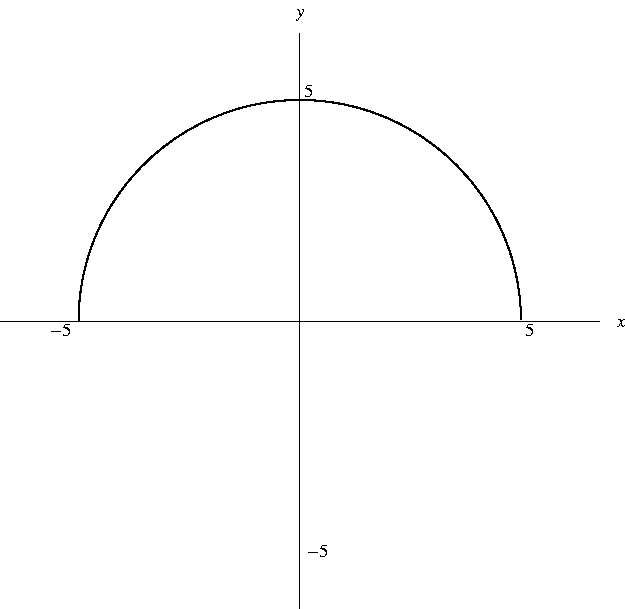
\includegraphics[height=2.5cm]{implicit-differentiation/pictures/03-06-circletop.pdf}%
}%
\ \uncover<4->{%
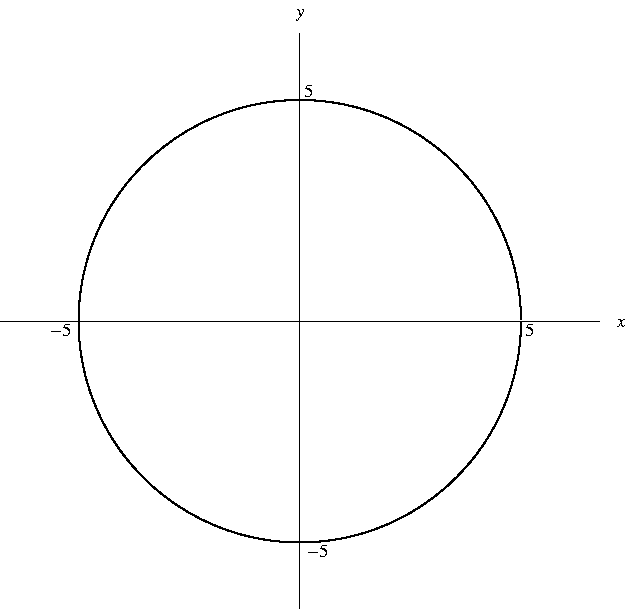
\includegraphics[height=2.5cm]{implicit-differentiation/pictures/03-06-circle.pdf}%
}%
\ \uncover<5->{%
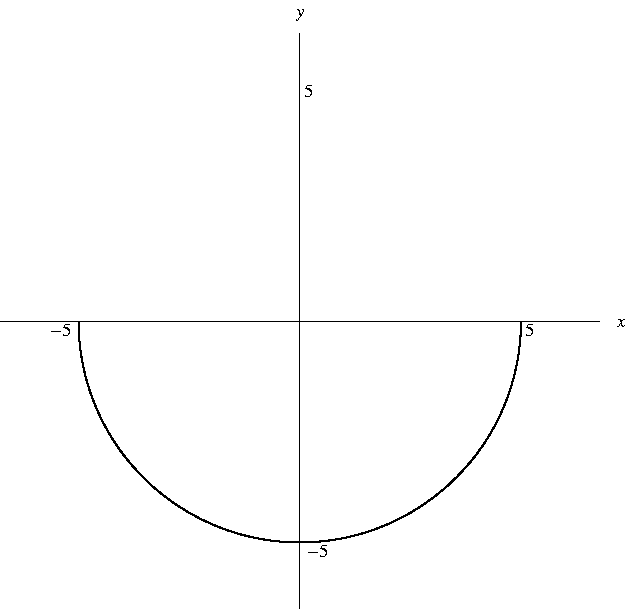
\includegraphics[height=2.5cm]{implicit-differentiation/pictures/03-06-circlebottom.pdf}%
}%
\end{center}
\end{frame}
% end module implicit-differentiation-intro
